\renewcommand{\NomeBloco}{\emph{Seletor 4x1}}
\renewcommand{\NomeBlocoNoIt}{Seletor 4x1}
\renewcommand{\NomePTab}{tab_\NomeBlocoNoIt}
\renewcommand{\NomeSTab}{tab_\NomeBlocoNoIt2}
\renewcommand{\NomePFig}{fig_\NomeBlocoNoIt}
\renewcommand{\NomeSFig}{fig_\NomeBlocoNoIt2}
\renewcommand{\NomeTTab}{tab_\NomeBlocoNoIt3}

\section{Seletor 4x1}

O bloco \NomeBloco{}\footnote{Circuito disponibilizado por Dalton Martini Colombo, orientador do trabalho aqui apresentado} tem a finalidade de selecionar uma entrada, e a colocar na sa\'ida. A entrada \'e selecionada atrav\'es de 4 entradas de seleção, em que apenas uma deve estar em n\'ivel l\'ogico um por vez. A \autoref{\NomePTab} indica a Tabela Verdade do bloco. Embora tenha uma l\'ogica digital, o circuito permite entradas e sa\'idas anal\'ogicas.

\begin{table}[htbp]

\caption{Tabela Verdade do bloco \NomeBloco}%
\label{\NomePTab}
\centering
\begin{tabular}{ccccc}
    \toprule
    Sel1 & Sel2 & Sel3 & Sel4 & Out \\
    \midrule \midrule
    1 & 0 & 0 & 0 & In1 \\
    \midrule
    0 & 1 & 0 & 0 & In2 \\
    \midrule
    0 & 0 & 1 & 0 & In3 \\
    \midrule
    0 & 0 & 0 & 1 & In4 \\
    \midrule
    0 & 0 & 0 & 0 & Z \\
    \midrule
    X & X & X & X & X \\
\bottomrule

\end{tabular}
\fonte{Produzido pelo autor.}
\end{table}

O bloco apresenta as definições de sinais de entrada e sa\'ida referidos na \autoref{\NomeSTab}.

\begin{table}[htbp]
\caption{Sinais do bloco \NomeBloco}
\label{\NomeSTab}
\centering
\begin{tabular}{ccl}

    \toprule
    Sinal & Tipo    & Descrição        \\
    \midrule \midrule
    In1    & Entrada & Primeira entrada \\
    \midrule
    Sel1    & Entrada & Seleção de entrada In1 \\
    \midrule
    In2    & Entrada & Segunda entrada \\
    \midrule
    Sel2    & Entrada & Seleção de entrada In2 \\
    \midrule
    In3    & Entrada & Terceira entrada \\
    \midrule
    Sel3    & Entrada & Seleção de entrada In3 \\
    \midrule
    In4    & Entrada & Quarta entrada \\
    \midrule
    Sel4    & Entrada & Seleção de entrada In4 \\
    \midrule
    Out   & Saída   & Sinal de Sa\'ida selecionado   \\
    \bottomrule
\end{tabular}
\legend{Fonte: Produzido pelo autor}
\end{table}

O circuito projetado para o bloco \'e demonstrado na \autoref{\NomePFig}.

\begin{figure}[htb]
 \centering
    \centering
    \caption{Circuito CMOS projetado para o bloco \NomeBloco} \label{\NomePFig}
    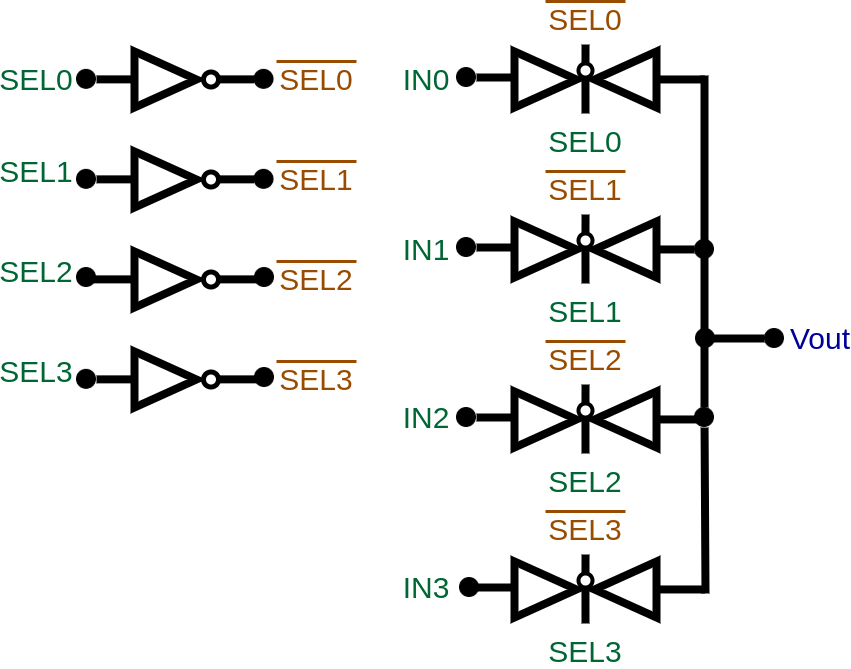
\includegraphics[scale=0.3]{Circuitos/sel4x1.png}
    \legend{Fonte: Produzido pelo autor}
\end{figure}

\begin{figure}[htb]
    \centering
    \caption{\label{\NomeSFig}Representação em bloco do \NomeBloco}
    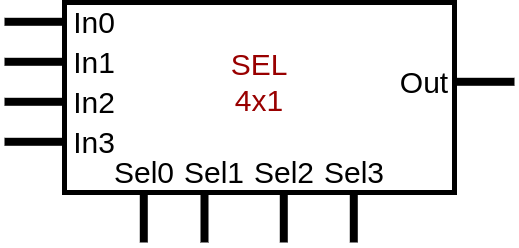
\includegraphics[scale=0.3]{Circuitos/sel4x1_block.png}
    \legend{Fonte: Produzido pelo autor}
\end{figure}

Os transistores utilizados no bloco \NomeBloco{} apresentam os par\^ametros mostrados na \autoref{\NomeTTab}.

\begin{table}[htbp]
\caption{Transistores do Bloco \NomeBloco}
\label{\NomeTTab}
\centering
\begin{tabular}{ccccc}
\toprule
Transistor & W ($\mu$m)  & L ($\mu$m)           & M (n° dispositivos) & S (n° dispositivos)\\
\midrule \midrule
Q1 & 1,2 & 0,18 & 1 & 1\\
\midrule
Q2 & 0,6 & 0,18 & 1 & 1\\
\bottomrule
\end{tabular}
\legend{Fonte: Produzido pelo autor}
\end{table}